\documentclass[10pt,twoside,reqno]{article}
\usepackage[marginparsep=1em]{geometry}
\geometry{lmargin=1.0in,rmargin=1.0in, bmargin=0.75in,  tmargin=0.75in}
\usepackage[usenames,dvipsnames,svgnames,table]{xcolor}
\usepackage{graphicx}
\usepackage{amssymb}
\usepackage{epstopdf}
\usepackage{tikz}
\usepackage{enumerate}
\usepackage{amsthm}
\usepackage{pgfplots}
\usepackage{tikz-3dplot}
\usetikzlibrary{shapes.geometric}
\usepackage{float}
\usepackage{amsmath}
\usepackage{fancyhdr}
\usepackage{lmodern}
\usepackage{chngcntr}
\usepackage{multicol, comment}

\pagestyle{fancy}
\fancyhf{}
\renewcommand{\sectionmark}[1]{\markright{\thesection.\ #1}}
\lhead{\fancyplain{}{}} 
\fancyhead[RE,RO]{MATH 2270}
\fancyfoot[RE,LO]{Dr. Heavilin}
\fancyfoot[LE,RO]{\thepage}


\begin{document}
\begin{flushright}
\begin{minipage}{.25\textwidth}
Dustin Ginos: \\
A01233669\\
Chandler Kinch: \\
A01662772\\
Jeff Wasden: \\
A01657029\\

\today
\end{minipage}
\end{flushright}

\center{\textbf{\underline{Homework 5}}}\\
\vspace{5mm}
\textbf{Chapter 5.1}
\begin{enumerate}
\item[5.1.3] True or false, with a reason if true or a counterexample if false: \\
{\addtolength{\leftskip}{10mm}
(a) The determinant of $I+A$ is $1$ + det$A$. \\ \vspace{2mm}
%~~~~~~~~~~~~~~~~~~~~~ ANSWER TO 5.1.3a ~~~~~~~~~~~~~~~~~~~~~~~~
\hspace{3mm}
False,
\hspace{5mm}
$
A=
\begin{bmatrix}
7&1&3\\
0&4&7\\
0&0&1\\
\end{bmatrix}
$
\hspace{5mm}
$
A+I=
\begin{bmatrix}
8&1&3\\
0&5&7\\
0&0&2\\
\end{bmatrix}
$
\hspace{5mm}
$1+|A|=29\neq|I+A|=80$ \\ \vspace{3mm}
%~~~~~~~~~~~~~~~~~~~~~~~~~~~~~~~~~~~~~~~~~~~~~~~~~~~~~~~~~~~~~~ 
(b) The determinant of $ABC$ is $|A||B||C|$. \\ \vspace{2mm}
%~~~~~~~~~~~~~~~~~~~~~ ANSWER TO 5.1.3b ~~~~~~~~~~~~~~~~~~~~~~~~
\hspace{3mm}
True, because of property \#9. \\
\vspace{3mm}
%~~~~~~~~~~~~~~~~~~~~~~~~~~~~~~~~~~~~~~~~~~~~~~~~~~~~~~~~~~~~~~ 
(c) The determinant of 4$A$ is $4|A|$. \\ \vspace{2mm}
%~~~~~~~~~~~~~~~~~~~~~ ANSWER TO 5.1.3c ~~~~~~~~~~~~~~~~~~~~~~~~
\hspace{3mm}
False, det
$
\left(4
\begin{bmatrix}
2&0\\
0&2\\
\end{bmatrix} \right)
= 8*8
$
 $\neq$ 
$
4
\begin{vmatrix}
2&0\\
0&2\\
\end{vmatrix}
= 4*4
$. \\
\vspace{3mm}
%~~~~~~~~~~~~~~~~~~~~~~~~~~~~~~~~~~~~~~~~~~~~~~~~~~~~~~~~~~~~~~ 
(d) The determinant of $AB-BA$ is zero. Try an example with 
$
A= 
\begin{bmatrix}
0&0\\
0&1\\
\end{bmatrix}
$. \\
%~~~~~~~~~~~~~~~~~~~~~ ANSWER TO 5.1.3d ~~~~~~~~~~~~~~~~~~~~~~~~
\hspace{3mm}
False, 
\hspace{5mm}
$
A=
\begin{bmatrix}
0&0\\
0&1\\
\end{bmatrix}
$
\hspace{5mm}
$
B=
\begin{bmatrix}
0&1\\
1&0\\
\end{bmatrix}
$ \\
\hspace{10mm}
$AB-BA=
\begin{bmatrix}
0&-1\\
1&0\\
\end{bmatrix}
$
 which is invertible, meaning the determinant is not zero. \\
\vspace{3mm}
%~~~~~~~~~~~~~~~~~~~~~~~~~~~~~~~~~~~~~~~~~~~~~~~~~~~~~~~~~~~~~~ 
}

\item[5.1.24] Elimination reduces $A$ to $U$. Then $A = LU$: \\
\begin{center}
$
A=
\begin{bmatrix}
3&3&4\\
6&8&7\\
-3&5&-9\\
\end{bmatrix}
=
\begin{bmatrix}
1&0&0\\
2&1&0\\
-1&4&1\\
\end{bmatrix}
\begin{bmatrix}
3&3&4\\
0&2&-1\\
0&0&-1\\
\end{bmatrix}
=LU
$. \\
\end{center}
Find the determinants of $L,U,A,U^{-1},L^{-1}, and U^{-1}L^{-1}A$. \\
%~~~~~~~~~~~~~~~~~~~~~ ANSWER TO 5.1.24 ~~~~~~~~~~~~~~~~~~~~~~~~
\vspace{2mm}
{\addtolength{\leftskip}{10mm}
If one reduces $L$ to its reduced row echelon form it becomes $I$. So $|L|=1$ \\ \vspace{2mm}
$|U|=3*2*-1=-6$ \\ \vspace{2mm}
$|A|=|U|=-6$ \\ \vspace{2mm}
$|U^{-1}L^{-1}|=\frac{1}{|U|}*\frac{1}{|L|}=-\frac{1}{6}$ \\ \vspace{2mm}
$|U^{-1}L^{-1}A|=|A|=1$ \\ \vspace{3mm}
}
%~~~~~~~~~~~~~~~~~~~~~~~~~~~~~~~~~~~~~~~~~~~~~~~~~~~~~~~~~~~~~~~ 

\item[5.1.27] Compute the determinants of these matrices by row operations: \\
\vspace{1mm}
\begin{center}
$
A=
\begin{bmatrix}
0&a&0\\
0&0&b\\
c&0&0\\
\end{bmatrix}
$
\hspace{8mm}
and
\hspace{8mm}
$
B=
\begin{bmatrix}
0&a&0&0\\
0&0&b&0\\
0&0&0&c\\
d&0&0&0\\
\end{bmatrix}
$
\hspace{8mm}
and
\hspace{8mm}
$
C=
\begin{bmatrix}
a&a&a\\
a&b&b\\
a&b&c\\
\end{bmatrix}
$. \\
\end{center}
%~~~~~~~~~~~~~~~~~~~~~ ANSWER TO 5.1.27 ~~~~~~~~~~~~~~~~~~~~~~~~
$A$: Two row swaps are required to get $A$ in the form 
$
\begin{bmatrix}
a&0&0\\
0&b&0\\
0&0&c\\
\end{bmatrix}
$
 so $|A|=(-1)(-1)abc=abc$. \\ \vspace{1mm}
$B$: Three row swaps are required to get $B$ in the form 
$
\begin{bmatrix}
d&0&0&0\\
0&a&0&0\\
0&0&b&0\\
0&0&0&c\\
\end{bmatrix}
$
\\ \hspace{10mm} so $|B|=(-1)(-1)(-1)abcd=abcd$. \\ \vspace{1mm}
$C$: You get RREF($C$) as  
$
\begin{bmatrix}
a&0&0\\
0&b-a&0\\
0&0&c-b\\
\end{bmatrix}
$
 so $|C|=a(b-a)(c-b)$. \\
\vspace{3mm}
%~~~~~~~~~~~~~~~~~~~~~~~~~~~~~~~~~~~~~~~~~~~~~~~~~~~~~~~~~~~~~~~

\item[5.1.28] True or false (give a reason if true or a 2 by 2 example if false):\\
{\addtolength{\leftskip}{10mm}
(a) If $A$ is not invertible then $AB$ is not invertible. \\ \vspace{2mm}
%~~~~~~~~~~~~~~~~~~~~~ ANSWER TO 5.1.28a ~~~~~~~~~~~~~~~~~~~~~~~~
\hspace{3mm}
True, det($AB$)=det($A) * $det($B$)=$0*$det($B$)=0. \\ \vspace{3mm}
%~~~~~~~~~~~~~~~~~~~~~~~~~~~~~~~~~~~~~~~~~~~~~~~~~~~~~~~~~~~~~~~
(b) The determinant of $A$ is always the products of its pivots. \\ \vspace{2mm}
%~~~~~~~~~~~~~~~~~~~~~ ANSWER TO 5.1.28b ~~~~~~~~~~~~~~~~~~~~~~~~
\hspace{3mm}
False, 
$
\begin{bmatrix}
0&1\\
1&0\\
\end{bmatrix}
$
 requires a row swap therefore the product is the products of its pivots times -1. \\ \vspace{2mm}
%~~~~~~~~~~~~~~~~~~~~~~~~~~~~~~~~~~~~~~~~~~~~~~~~~~~~~~~~~~~~~~~
(c) The determinant of $A-B$ equals det($A$) - det($B$). \\ \vspace{2mm}
%~~~~~~~~~~~~~~~~~~~~~ ANSWER TO 5.1.28c ~~~~~~~~~~~~~~~~~~~~~~~~
\hspace{3mm}
False, 
$
\left|
\begin{bmatrix}
1&0\\
1&1\\
\end{bmatrix}
 - 
\begin{bmatrix}
0&-1\\
0&0\\
\end{bmatrix}
\right|
=
\begin{vmatrix}
1&1\\
1&1\\
\end{vmatrix}
=0 \neq
\begin{vmatrix}
1&0\\
1&1\\
\end{vmatrix}
 - 
\begin{vmatrix}
0&-1\\
0&0\\
\end{vmatrix}
=1-0=1
$ \\ \vspace{2mm}
%~~~~~~~~~~~~~~~~~~~~~~~~~~~~~~~~~~~~~~~~~~~~~~~~~~~~~~~~~~~~~~~
(d) $AB$ and $BA$ have the same determinant. \\ \vspace{2mm}
%~~~~~~~~~~~~~~~~~~~~~ ANSWER TO 5.1.28d ~~~~~~~~~~~~~~~~~~~~~~~~
\hspace{3mm}
True, since multiplication is commutative. $|AB|=|A||B|=|B||A|=|BA|$ \\ \vspace{2mm}
%~~~~~~~~~~~~~~~~~~~~~~~~~~~~~~~~~~~~~~~~~~~~~~~~~~~~~~~~~~~~~~~
}
\end{enumerate}
\vspace{5mm}
\textbf{Chapter 5.2}
\begin{enumerate}
\item[5.2.9] Show that 4 is the largest determinant for a 3 by 3 matrix of 1's and -1's. \\
%~~~~~~~~~~~~~~~~~~~~~ ANSWER TO 5.2.9 ~~~~~~~~~~~~~~~~~~~~~~~~
\vspace{3mm}

The determinant for a 3x3 matrix has six terms, half of which are positive. Each value from the matrix is a part of two of those terms, once in a positive and once in a negative term. If all values were all positive 1's or negative 1's the determinant would be three. If there are an even number of negative 1's then the largest the determinant could be and would be is four.

\vspace{3mm}
%~~~~~~~~~~~~~~~~~~~~~~~~~~~~~~~~~~~~~~~~~~~~~~~~~~~~~~~~~~~~~~

\item[5.2.23] With 2 by 2 blocks in 4 by 4 matrices, you cannot always use block determinants: \\
\begin{center}
$
\begin{vmatrix}
A&B\\
0&D\\
\end{vmatrix}
=
\begin{vmatrix}
A\\
\end{vmatrix}
\begin{vmatrix}
D\\
\end{vmatrix}
$
\hspace{10mm}
$
\begin{vmatrix}
A&B\\
C&D\\
\end{vmatrix}
\neq
\begin{vmatrix}
A\\
\end{vmatrix}
\begin{vmatrix}
D\\
\end{vmatrix}
-
\begin{vmatrix}
C\\
\end{vmatrix}
\begin{vmatrix}
B\\
\end{vmatrix}
$. \\
\end{center}
{\addtolength{\leftskip}{10mm}
(a) Why is the first statement true? Somehow $B$ doesn't enter. \\ \vspace{2mm}
%~~~~~~~~~~~~~~~~~~~~~ ANSWER TO 5.2.23a ~~~~~~~~~~~~~~~~~~~~~~~~
\hspace{3mm} Any entry from $B$ times any entry from the zero block is zero, so $B$ can be excluded. \\
\vspace{3mm}
%~~~~~~~~~~~~~~~~~~~~~~~~~~~~~~~~~~~~~~~~~~~~~~~~~~~~~~~~~~~~~~~ 
(b) Show by example that equality fails (as shown) when $C$ enters. \\ \vspace{2mm}
%~~~~~~~~~~~~~~~~~~~~~ ANSWER TO 5.2.23b ~~~~~~~~~~~~~~~~~~~~~~~~
\begin{center}
$
A=
\begin{bmatrix}
1&0\\
0&0\\
\end{bmatrix}
\hspace{5mm}
B=
\begin{bmatrix}
0&0\\
1&0\\
\end{bmatrix}
\hspace{5mm}
C=
\begin{bmatrix}
0&1\\
0&0\\
\end{bmatrix}
\hspace{5mm}
D=
\begin{bmatrix}
0&0\\
0&1\\
\end{bmatrix}
$
 \\
$
|A||D|-|C||B|=0\neq
\begin{vmatrix}
1&0&0&0\\
0&0&1&0\\
0&1&0&0\\
0&0&0&1\\
\end{vmatrix}
= -1
$ \\
\end{center}
%~~~~~~~~~~~~~~~~~~~~~~~~~~~~~~~~~~~~~~~~~~~~~~~~~~~~~~~~~~~~~~~ 
(c) Show by example that the answer det($AD-CB$) is also wrong. \\ \vspace{2mm}
}
%~~~~~~~~~~~~~~~~~~~~~ ANSWER TO 5.2.23c ~~~~~~~~~~~~~~~~~~~~~~~~
\begin{center}
det
$
\left(
\begin{bmatrix}
1&0\\
0&0\\
\end{bmatrix}
\begin{bmatrix}
0&0\\
1&0\\
\end{bmatrix}
-
\begin{bmatrix}
0&1\\
0&0\\
\end{bmatrix}
\begin{bmatrix}
0&0\\
0&1\\
\end{bmatrix}
\right)
=
$
det
$
\left(
\begin{bmatrix}
0&0\\
0&0\\
\end{bmatrix}
-
\begin{bmatrix}
0&1\\
0&0\\
\end{bmatrix}
\right)
\neq
\begin{vmatrix}
A&B\\
C&D\\
\end{vmatrix}
= -1
$ \\
\end{center}
%~~~~~~~~~~~~~~~~~~~~~~~~~~~~~~~~~~~~~~~~~~~~~~~~~~~~~~~~~~~~~~~ 

\item[5.2.33] The symmetric Pascal matrices have determinant 1. If I subtract 1 from the $n, n$ entry, why does the determinant become zero? (Use rule 3 or cofactors.) \\
\begin{center}
det
$
\begin{bmatrix}
1&1&1&1\\
1&2&3&4\\
1&3&6&10\\
1&4&10&20\\
\end{bmatrix}
=1
$
 (known)
\hspace{12mm}
det
$
\begin{bmatrix}
1&1&1&1\\
1&2&3&4\\
1&3&6&10\\
1&4&10&\textbf{19}\\
\end{bmatrix}
=\textbf{0}
$
 (to explain). \\
\end{center}
%~~~~~~~~~~~~~~~~~~~~~ ANSWER TO 5.2.33 ~~~~~~~~~~~~~~~~~~~~~~~~
\vspace{2mm}
\begin{center}
$
\begin{vmatrix}
1&1&1&1\\
1&2&3&4\\
1&3&6&10\\
1&4&10&19\\
\end{vmatrix}
=
\begin{vmatrix}
1&1&1&1\\
1&2&3&4\\
1&3&6&10\\
1&4&10&20\\
\end{vmatrix}
+
\begin{vmatrix}
1&1&1&1\\
1&2&3&4\\
1&3&6&10\\
0&0&0&-1\\
\end{vmatrix}
= 1 + (-1) = 0
$
\end{center}
\vspace{3mm}
%~~~~~~~~~~~~~~~~~~~~~~~~~~~~~~~~~~~~~~~~~~~~~~~~~~~~~~~~~~~~~~~ 
\end{enumerate}
\vspace{5mm}
\textbf{Chapter 5.3}
\begin{enumerate}
\item[5.3.16] (a) Find the area of the parallelogram with edges $v = (3, 2)$ and $w = (1, 4)$ \\
%~~~~~~~~~~~~~~~~~~~~~ ANSWER TO 5.3.16 ~~~~~~~~~~~~~~~~~~~~~~~~
\vspace{3mm}
area $= \begin{vmatrix}
3 & 2\\
1 & 4\\
\end{vmatrix}
= 12 - 2 = 10
$\\
\vspace{3mm}
%~~~~~~~~~~~~~~~~~~~~~~~~~~~~~~~~~~~~~~~~~~~~~~~~~~~~~~~~~~~~~~~ 
(b) Find the area of the triangle with sides $v, w$, and $v + w$. Draw it.\\
%~~~~~~~~~~~~~~~~~~~~~ ANSWER TO 5.3.16 ~~~~~~~~~~~~~~~~~~~~~~~~
\vspace{3mm}
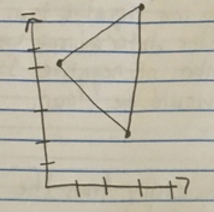
\includegraphics[scale=1]{(b).png} area$ = \frac{1}{2}\begin{vmatrix}
3&2&1\\
1&4&1\\
4&6&1\\
\end{vmatrix} = \frac{1}{2}(3(-2) + 2(3) - 10) = -5 = \lvert -5 \rvert = 5$\\
\vspace{3mm}
%~~~~~~~~~~~~~~~~~~~~~~~~~~~~~~~~~~~~~~~~~~~~~~~~~~~~~~~~~~~~~~~ 
(c) find the area of the triangle with sides $v, w$, and $w - v$. Draw it\\
%~~~~~~~~~~~~~~~~~~~~~ ANSWER TO 5.3.16 ~~~~~~~~~~~~~~~~~~~~~~~~
\vspace{3mm}
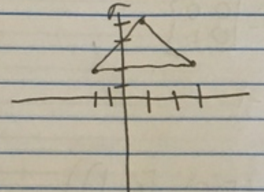
\includegraphics[scale=1]{(c).png} area = $\frac{1}{2} \begin{vmatrix}
3&2&1\\
1&4&1\\
-2&2&1\\
\end{vmatrix} = \frac{1}{2}(3(2) + 2(-3) -10) = -5 = \lvert -5 \rvert = 5$\\
\vspace{3mm}
%~~~~~~~~~~~~~~~~~~~~~~~~~~~~~~~~~~~~~~~~~~~~~~~~~~~~~~~~~~~~~~~ 
\item[5.3.20]The Hadamard matrix $H$ has orthogonal rows. The box is hypercube!\\
\begin{center}
What is
$
$$
\lvert
H
\rvert
=
\begin{vmatrix}
1&1&1&1\\
1&1&-1&-1\\
1&-1&-1&1\\
1&-1&1&-1\\
\end{vmatrix}
= $ volume of a hypercube in $ R^4
$$
$
\end{center}
%~~~~~~~~~~~~~~~~~~~~~ ANSWER TO 5.3.20 ~~~~~~~~~~~~~~~~~~~~~~~~
\vspace{3mm}
$
$$
\begin{vmatrix}
1&1&1&1\\
1&1&-1&-1\\
1&-1&-1&1\\
1&-1&1&-1\\
\end{vmatrix}
=
\begin{vmatrix}
1&1&1&1\\
0&0&-2&-2\\
0&-2&-2&0\\
0&-2&0&-2\\
\end{vmatrix}
=
-
\begin{vmatrix}
1&1&1&1\\
0&-2&-2&0\\
0&0&-2&-2\\
0&-2&0&-2\\
\end{vmatrix}
=
-
\begin{vmatrix}
1&1&1&1\\
0&-2&-2&0\\
0&0&-2&-2\\
0&0&2&-2\\
\end{vmatrix}
=
\begin{vmatrix}
1&1&1&1\\
0&-2&-2&0\\
0&0&-2&-2\\
0&0&0&-4\\
\end{vmatrix}
$$
$\\
\vspace{2mm}
$= 1 \cdot -2 \cdot -2 \cdot -4 = 16$\\

\vspace{3mm}
%~~~~~~~~~~~~~~~~~~~~~~~~~~~~~~~~~~~~~~~~~~~~~~~~~~~~~~~~~~~~~~~
\item[5.3.21] If the columns of a 4 by 4 matrix have lengths $L_1, L_2, L_3, L_4$, what is the largest possible value for the determinant (based on volumne)? If all entries of the matrix are 1 or -1, what are those lengths and the maximum determinant?\\
%~~~~~~~~~~~~~~~~~~~~~ ANSWER TO 5.3.21 ~~~~~~~~~~~~~~~~~~~~~~~~
\vspace{3mm}
$
$$
\begin{vmatrix}
1&1&1&1\\
1&1&-1&-1\\
1&-1&-1&1\\
1&-1&1&-1\\
\end{vmatrix}
$$
$\\
\vspace{2mm}
$L_1 = (1, 1, 1, 1)$, $L_2 = (1, 1, -1, -1)$, $L_3 = (1, -1, -1, 1)$, $L_4 = (1, -1, 1, -1)$\\
max det $= 16$\\

\vspace{3mm}
%~~~~~~~~~~~~~~~~~~~~~~~~~~~~~~~~~~~~~~~~~~~~~~~~~~~~~~~~~~~~~~~  
\item[5.3.27] Polar coordinates satisfy $x = rcos\theta$ and $y = rsin\theta$. Polar area is $J$ $dr$ $d\theta$:\\
\begin{center}
$
$$
J =
\begin{vmatrix}
\frac{\partial x}{\partial r} & \frac{\partial x}{\partial \theta}\\
\frac{\partial y}{\partial r} & \frac{\partial y}{\partial \theta}\\
\end{vmatrix}
=
\begin{vmatrix}
cos\theta & -rsin\theta\\
sin\theta & rcos\theta\\
\end{vmatrix}
$$
$\\
\end{center}
The two columns are orthogonal. Their lengths are \underline{\hspace{7mm}}. Thus $J =$ \underline{\hspace{7mm}}.\\
%~~~~~~~~~~~~~~~~~~~~~ ANSWER TO 5.3.27 ~~~~~~~~~~~~~~~~~~~~~~~~
\vspace{3mm}
$1$ and $r$, $J = r$\\
\vspace{3mm}
%~~~~~~~~~~~~~~~~~~~~~~~~~~~~~~~~~~~~~~~~~~~~~~~~~~~~~~~~~~~~~~~ 
\item[5.3.28] Spherical coordinates $\rho, \phi, \theta$ satisfy $x = \rho sin \phi cos \theta$ and $y = \rho sin \phi sin \theta$ and $z = \rho cos \phi$. Find the 3 by 3 matrix of partial derivatives: $\partial x$/$\partial \rho$, $\partial x$/$\partial \phi$, $\partial x$/$\partial \theta$ in row 1. Simplify its determinant to $J = \rho^2 sin \phi$. Then $dV$ in spherical coordinates is $\rho^2sin\phi dp d\phi d \theta$, the volume of an infinitesimal "coordinate box".\\
%~~~~~~~~~~~~~~~~~~~~~ ANSWER TO 5.3.28 ~~~~~~~~~~~~~~~~~~~~~~~~
\vspace{3mm}
$
$$
J =
\begin{vmatrix}
sin\phi cos\theta & \rho cos \phi cos \theta & -\rho sin \phi sin \theta\\
sin\phi sin\theta & \rho cos \phi sin \theta & \rho sin \phi cos \theta\\
cos\theta & -\rho sin \phi & 0\\
\end{vmatrix}
= \rho ^2 sin\phi
$$
$


\vspace{3mm}
%~~~~~~~~~~~~~~~~~~~~~~~~~~~~~~~~~~~~~~~~~~~~~~~~~~~~~~~~~~~~~~~ 
\item[5.3.29] The matrix that connects $r, \theta$ to $x, y$ is Problem 27. Invert that 2 by 2 matrix:\\
\begin{center}
$
$$
J^{-1} =
\begin{vmatrix}
\frac{\partial r}{\partial x} & \frac{\partial r}{\partial y}\\
\frac{\partial \theta}{\partial x} & \frac{\partial \theta}{\partial y}\\
\end{vmatrix}
=
\begin{vmatrix}
cos\theta & ?\\
? & ?\\
\end{vmatrix}
= ?
$$
$\\
\end{center}
If is surprising that $\partial r$/$\partial x = \partial x$/$\partial r$ (Calculus, Gilbert Strang, p. 501). Multiplying the matrices $J$ and $J^{-1}$ gives the chain rule $\frac{\partial x}{\partial x} = \frac{\partial x}{\partial r}\frac{\partial r}{\partial x} + \frac{\partial x}{\partial \theta}\frac{\partial \theta}{
\partial x} = 1$.\\
%~~~~~~~~~~~~~~~~~~~~~ ANSWER TO 5.3.29~~~~~~~~~~~~~~~~~~~~~~~~
\vspace{3mm}
$
$$
J^{-1}
=
\begin{vmatrix}
cos\theta & sin \theta\\
\frac{-sin\theta}{r} & \frac{cos\theta}{r}\\
\end{vmatrix}
=
\frac{1}{r}cos^2\theta + \frac{1}{r}cos^2\theta = \frac{1}{r}
$$
$\\


\vspace{3mm}
%~~~~~~~~~~~~~~~~~~~~~~~~~~~~~~~~~~~~~~~~~~~~~~~~~~~~~~~~~~~~~~~ 
\end{enumerate}
\end{document}  